\section{Experiments}\label{sec_equiv:experiments}

We consider two different setups. The conventional compressed sensing discussed in section \ref{sec:related_gen_cs} (no rotation) and compressed sensing with unknown orientation discussed in section \ref{sec:gen_cs_rotation} (unknown rotation).  

\paragraph{Datasets}
We conduct experiments on two different datasets. We start with benchmarking experiments on MNIST. 
Subsequently, concerning a real-world application of the proposed approach, we conduct experiments on the Low Dose CT Image and Projection Data\footnote{\url{https://www.aapm.org/grandchallenge/lowdosect/}} (MAYO) dataset \citep{moen2021low}, which consist of three types of data: DICOM-CT-PD projection data, DICOM image data, and Excel clinical data reports. To our aim, we use the DICOM subset only. Images are divided into three sets labelled N for neuro, C for chest, and L for liver each of which comprises 512x512 images from 50 different patients. To train the generative priors, we consider the L subset which is made of $\sim$7K samples that we divide into train, validation and test sets comprising $\sim$80\%, $\sim$10\%, and $\sim$10\% of the images, respectively.
Before feeding a model, we randomly crop the image and then rescale it to 128x128, and finally, we normalize the pixels value in $[0,1]$.

\begin{figure}[t]
    \centering
    \begin{tabular}{ll}
        \multicolumn{1}{c}{No rotation}& \multicolumn{1}{c}{Unknown rotation}\\
        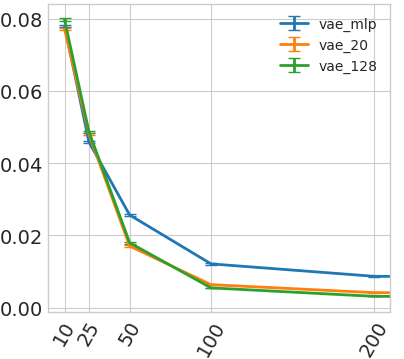
\includegraphics[width=0.39\textwidth]{pics/2_equiv_vae/vae_mse_no_rotation.png} &
        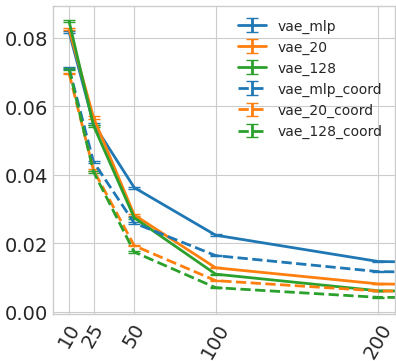
\includegraphics[width=0.39\textwidth]{pics/2_equiv_vae/vae_mse_unknown_rotation_copy.png} \\
        \multicolumn{1}{c}{Number of measurements} &
        \multicolumn{1}{c}{Number of measurements}\\
    \end{tabular}
    \caption[][\baselineskip]{Comparison of MLP-VAE and Convolutional VAE with the latent dimentions 20 and 128 on MNIST dataset. Average MSE for 10000 test points.}
    \label{fig:vae_prior_types}
    \vskip 0.1in
\end{figure}

\paragraph{Prior Generative Models}
We compare various generative models as prior on the signals that we aim to reconstruct. Broadly speaking, we consider two types of generative models in our experiments: VAE and Normalizing Flow. In the former case, we have MLP-VAE, fully convolutional VAE (Conv-VAE) and Equivariant VAE (Eq-VAE: proposed model). And in the latter, as a flow prior, we consider a multi-scale RealNVP model. To bring the non-equivariant models, i.e., flow and VAE, at par with the Eq-VAE in terms of their ability to generate rotated images so that they can be effectively used as a prior for CS with unknown rotation, we consider two routes, 1. Conditional model: we include a conditional flow (Cond. Flow) model, which has rotation angle as an additional input and is trained on the augmented (rotated) dataset, 2. Augmented models: another way to augment the capabilities of conventional generative models is to train them on augmented (rotated) datasets. On this line, we include augmented VAE (Aug-VAE), and augmented flow (Aug-Flow) as conventional VAE and Flow but explicitly trained on augmented (addition of random rotation as a pre-processing step) dataset. In our MNIST experiments, we noticed impractically high latency of Cond. Flow during both the generative prior training and the following CS experiment. The problem gets highly exacerbated for the MAYO dataset as it is more complex than MNIST, and hence, we decided to drop the Cond. Flow for MAYO due to its impractical latency.

% For the compressed sensing with the rotation we also add a conditional flow model, which has an additional input (rotation angle), which allows it to generate rotated images. Being the MAYO dataset more challenging than MNIST, we decide to train an augmented version for VAE and Flow (Aug-VAE and Aug-Flow) by explicitly adding random rotations as a data preprocessing step. 

\paragraph{Metrics}
When it comes to measuring the success of the compressed sensing, we are interested in two criteria: reconstruction quality and convergence speed. We measure MSE to evaluate the quality of the reconstruction. For convergence, we assume that if the MSE (per pixel) is lower than 0.01, then the reconstruction is successful. We then report the proportion of converged points and the average number of iterations (or gradient descent steps) required for a method to converge. 

\begin{table}[ht]
\caption[][\baselineskip]{CS results on MNIST. We report results averaged over 1000 test points. By Converged Points, we refer to points that, for a given number of iterations, resulted in MSE (per pixel) lower than $1.e^{-2}$. We emphasize in bold, results from the best model.}
\label{tab:mnist_cs_results}
\begin{center}
% \begin{sc}
\resizebox{\textwidth}{!}{
\begin{tabular}{lll|ccc|ccc|ccc}
% \begin{tabular}{\linewidth}{@{}lll|YYc|YYc|YYc@{}}
\toprule
&&\multirow{2}{*}{Prior} & \multicolumn{3}{c|}{50 measurements} & \multicolumn{3}{c|}{100 measurements} & \multicolumn{3}{c}{200 measurements} \\
&&& MSE & Converged  & \# iter$\downarrow$ &  MSE  & Converged  & \# iter$\downarrow$ &  MSE & Converged  & \# iter $\downarrow$\\ 
&&&  ($1.e^{-3}$)$\downarrow$ & Points (\%)$\uparrow$ &  &   ($1.e^{-3}$)$\downarrow$ & Converged  &  &  ($1.e^{-3}$)$\downarrow$ &  Points (\%)$\uparrow$ & \\ \midrule
&\multirow{5}{*}{\STAB{\rotatebox[origin=c]{90}{No rotation}}}
& Flow        & 45.4 & 100 & 59 & 19.2 & 100 & 39 & 10.2 & 100 & 38 \\
&& Cond. Flow & 22.6 & 100 & 35 & 10.1 & 100 & \textbf{22} & 5.8 & 100 & \textbf{22} \\
&& MLP-VAE    & 25.7 & 100 & 50 & 12.1 & 100 & 41 & 8.7 & 100 & 38\\
&& Conv-VAE   & 18.0 & 100 & 48 & 5.5  & 100 & 39 & 3.2 & 100 & 35\\
&& Eq-VAE     & \textbf{10.6} & 100 & \textbf{34} & \textbf{2.6}  & 100 & \textbf{22} & \textbf{2.1} & 100 & \textbf{22}\\ \midrule
\multirow{5}{*}{\STAB{\rotatebox[origin=c]{90}{Unknown}}}
& \multirow {5}{*}{\STAB{\rotatebox[origin=c]{90}{rotation}}}
& Flow        & 27.2 & 100 & 73 & 13.2 & 100 & 60 & 7.6  & 100 & 36 \\
&& Cond. Flow & 17.9 & 100 & 42 & 7.2  & 100 & 32 & 6.0  & 100 & 30 \\
&& MLP-VAE    & 25.9 & 100 & 48 & 16.4 & 100 & 40 & 11.7 & 100 & 34\\
&& Conv-VAE   & 17.5 & 100 & 51 & 7.0  & 100 & 39 & 4.2  & 100 & 32\\
&& Eq-VAE     & \textbf{11.8} & 100 & \textbf{33} & \textbf{4.2}  & 100 & \textbf{24} & \textbf{3.2}  & 100 & \textbf{23}\\
\bottomrule
\end{tabular}
}
% \end{sc}
\end{center}
% \vskip 0.2in
\vspace*{\baselineskip}
\end{table}


\subsection{Benchmark experiments on MNIST}
Concerning compressed sensing experiments, we consider a different number of linear measurements to reconstruct the input signal. Specifically, in \autoref{tab:mnist_cs_results} we report CS results for the MNIST dataset considering 50, 100, and 200 measurements. For each of the mentioned values, and each prior model, we report the average value for the MSE and the number of iterations required to achieve a 100\% success rate for reconstructing the input signals.
As mentioned previously, we consider two different scenarios: no rotations and unknown rotations. In both cases, Eq-VAE prior report the best performance concerning MSE and the number of iterations required to reconstruct the input images.
Indeed, although with all the priors we observe a 100\% convergence rate for the CS experiments, Eq-VAE requires fewer iterations and reports a lower average MSE than all the other models.

Following \cite{Bora2017-as} we train MLP-VAE with 20 dimensional latent space. However, as can be seen from the Figure \ref{fig:vae_prior_types}, fully convolutional VAE with the same latent space dimensionality tends to perform better both with and without rotation. Presumably, the introduction of the fully convolutional architecture makes the model equivariant to the translation, which is beneficial for the compressed sensing. As results in Table \ref{tab:mnist_cs_results} show, equivariance to rotation improves the performance even further. 

Figure \ref{fig:vae_prior_types} also shows that larger latent space of the convolutional VAE gives a slight performance improvement. Thus we chose to train equivariant prior with the same latent dimension. When rotation is unknown, we also compare coordinate gradient descent (\textit{dashed line}) with the joint optimization of the latent code and the rotation angle (\textit{solid line}). In all the experiments, coordinate gradient descent shows better results.
% (e.g. \cs{vae\_mlp\_coord} vs  \cs{vae\_mlp}).  #Arash

\begin{table}[t]
\caption[][\baselineskip]{CS results on MAYO. The reported results corresponding to 200 measurements. By Converged Points, we refer to points that, for a given number of iterations, resulted in MSE (per pixel) lower than $1.e^{-2}$. Concerning the MSE, we reported the mean value $\pm 1 \sigma$. The MSE is computed across converged points only. We emphasize in bold, results from the best model.}

\label{tab:mayo_cs_results}
\begin{center}
\resizebox{\textwidth}{!}{
\begin{tabular}{lll|cc|cc|cc|cc}
% \begin{tabularx}{\linewidth}{@{}lll|YY|YY|YY|YY@{}}
\toprule
&&\multirow{2}{*}{Prior} & \multicolumn{2}{c|}{50 iterations} & \multicolumn{2}{c|}{100 iterations} & \multicolumn{2}{c|}{150 iterations} & \multicolumn{2}{c}{200 iterations} \\
&&& MSE  & Converged  &  MSE  & Converged   &  MSE & Converged  &  MSE  & Converged \\
&&& ($1.e^{-3}$)$\downarrow$ & Points (\%)$\uparrow$  &  ($1.e^{-3}$)$\downarrow$ & Points (\%)$\uparrow$  &   ($1.e^{-3}$)$\downarrow$ & Points (\%)$\uparrow$  &  ($1.e^{-3}$)$\downarrow$ & Points (\%)$\uparrow$ \\ \midrule
&\multirow{5}{*}{\STAB{\rotatebox[origin=c]{90}{No rotation}}}
& Flow & 8.9 $\pm$ 0.9 & 28.2 & 8.1 $\pm$ 1.2 & 65.9 & 7.3 $\pm$ 1.3 & 79.7 & 6.8 $\pm$ 1.4  & 86.8  \\
&& Aug-Flow & N/A & 0.0 & 8.2 $\pm$ 1.2 & 40.1 & 7.4 $\pm$ 1.4 & 77.1 & 6.7 $\pm$ 1.4 & 83.4 \\
&& Conv-VAE & 7.9 $\pm$ 1.3 & 39.9 & 6.8 $\pm$ 1.6 & 76.2 & 6.2 $\pm$ 1.8 & \bf{89.6} & 5.9 $\pm$ 1.8  & \bf{95.5}  \\
&& Aug-VAE & 7.5 $\pm$ 1.3 & 51.7 & \bf{6.1 $\pm$ 1.6} & 75.7 & \bf{5.7 $\pm$ 1.7} & 83.8 & \bf{5.5 $\pm$ 1.6}  & 88.1  \\
&& Eq-VAE &  \bf{7.4 $\pm$ 1.4} & \bf{73.5} & 6.4 $\pm$ 1.4 & \bf{86.9} & 6.1 $\pm$ 1.5  & 89.2  & 6.0 $\pm$ 1.5  & 90.4  \\ \midrule
\multirow{5}{*}{\STAB{\rotatebox[origin=c]{90}{Unknown}}}
& \multirow{5}{*}{\STAB{\rotatebox[origin=c]{90}{rotation}}}
& Flow & 7.2 $\pm$ 1.4 & \bf{76.4} & \bf{5.8 $\pm$ 1.5} & 83.8 & \bf{5.2 $\pm$ 1.6} & 87.5 & \bf{5.0 $\pm$ 1.7} & \bf{93.3}  \\
&& Aug-Flow & N/A & 0.0 & 8.2 $\pm$ 1.1 & 49.9 & 6.9 $\pm$ 1.3 & 80.9 & 6.0 $\pm$ 1.3 & 84.3 \\
&& Conv-VAE & \bf{7.1 $\pm$ 1.7} & 55.3 & 5.9 $\pm$ 2.1 & 80.5 & 5.4 $\pm$ 2.1 & 88.2 & 5.0 $\pm$ 2.0  & 90.2 \\
&& Aug-VAE & 7.5 $\pm$ 1.5 & 59.3 & 5.9 $\pm$ 1.6 & 85.2 & 5.3 $\pm$ 1.5 & 89.1 & 5.1 $\pm$ 1.6  & 92.4  \\
&& Eq-VAE &  7.6 $\pm$ 1.4 & 70.3 & 6.6 $\pm$ 1.5 & \bf{87.5} & 6.1 $\pm$ 1.5 & \bf{91.3} & 6.0 $\pm$ 1.6 & 92.7  \\ \midrule
\bottomrule
% \end{tabularx}
\end{tabular}
}
\end{center}
\vspace*{\baselineskip}
\end{table}


\subsection{CT scans reconstruction: MAYO dataset}
We report in~\autoref{tab:mayo_cs_results} results for the MAYO dataset. Differently from the MNIST result, in this case, we fix the number of measurements to 200 and evaluate the performance of the different generative priors on the CS task considering a different number of iterations. Specifically, we consider 50, 100, 150, and 200 iterations, and for each of them, we report the average MSE and the percentage of points successfully reconstructed (i.e., with MSE per pixel below 0.01). 
Being the MAYO dataset more complex than the MNIST, in this case, we do not observe a clear dominance of one type of prior compared to the others. However, as a general remark, we can notice that using Eq-VAE the average percentage of converged points is higher than for other models for both no rotations, 85.0\%, and unknown rotations, 85.5\%. As a comparison, the second-best performing priors are the VAE with 75.3\%, and the Flow with 85.2\%, concerning no and unknown rotations, respectively. 
Instead, regarding the MSE, all the results agree within 1 standard deviation.

\begin{figure}[!ht]
    \centering
    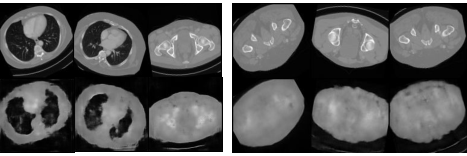
\includegraphics[width=\linewidth]{pics/2_equiv_vae/eqvae_vae_cs_recon_unk_rot.pdf}\hfill
    \caption{Example of reconstructed images using Eq-VAE (left-3) and VAE (right-3) as a prior. The top row shows ground truth rotated images prior to measurement, and the bottom row shows the corresponding CS reconstructed images. We notice in the third column (both left and right images), the VAE reconstructed image is $180^{\circ}$ rotated with respect to the canonical configuration while the Eq. VAE is able to retrieve the configuration effectively.}
    \label{fig:mayo_eqvae_vae_rec_unk}
\end{figure}


\subsection{Discussion}
As we discussed before, the upper bound on the reconstruction error in Theorem \ref{thm:equivmodel} suggests that there is no difference in the performance of equivariant models in rotated and non-rotated cases. The results for the MAYO dataset show a small performance drop from no rotation to unknown rotation cases. The discrepancy is a bit larger for MNIST experiments. 
The difference can be attributed to the fact that equivariant models are built for finite rotation groups while we test on continuous rotation groups. 
In Figure~\ref{fig:mayo_eqvae_vae_rec_unk} we report a comparison between reconstructed rotated samples from Eq-VAE(left) and VAE (right). As expected, Eq-VAE successfully recovers the correct orientation for the reconstructed images while VAE struggles to achieve such a goal. 

\paragraph{Group Choice} 
We train the equivariant prior under the action of the cyclic group. This is a discrete group, size of which, is a hyperparameter to choose. However, in our compressed sensing experiments with unknown orientation, the rotation angle is sampled uniformly. Thus, a larger group size will potentially lead to a better-compressed sensing performance. We compared three different group sizes (see Appendix \ref{appx:eq_vae_group}) and conclude that group $C_{16}$ results in the best reconstruction results in both the CS setups.
